% Options for packages loaded elsewhere
\PassOptionsToPackage{unicode}{hyperref}
\PassOptionsToPackage{hyphens}{url}
\documentclass[
  10pt,
  a4paper,
]{article}
\usepackage{xcolor}
\usepackage[margin=22mm]{geometry}
\usepackage{amsmath,amssymb}
\setcounter{secnumdepth}{-\maxdimen} % remove section numbering
\usepackage{iftex}
\ifPDFTeX
  \usepackage[T1]{fontenc}
  \usepackage[utf8]{inputenc}
  \usepackage{textcomp} % provide euro and other symbols
\else % if luatex or xetex
  \usepackage{unicode-math} % this also loads fontspec
  \defaultfontfeatures{Scale=MatchLowercase}
  \defaultfontfeatures[\rmfamily]{Ligatures=TeX,Scale=1}
\fi
\usepackage{lmodern}
\ifPDFTeX\else
  % xetex/luatex font selection
\fi
% Use upquote if available, for straight quotes in verbatim environments
\IfFileExists{upquote.sty}{\usepackage{upquote}}{}
\IfFileExists{microtype.sty}{% use microtype if available
  \usepackage[]{microtype}
  \UseMicrotypeSet[protrusion]{basicmath} % disable protrusion for tt fonts
}{}
\makeatletter
\@ifundefined{KOMAClassName}{% if non-KOMA class
  \IfFileExists{parskip.sty}{%
    \usepackage{parskip}
  }{% else
    \setlength{\parindent}{0pt}
    \setlength{\parskip}{6pt plus 2pt minus 1pt}}
}{% if KOMA class
  \KOMAoptions{parskip=half}}
\makeatother
\usepackage{graphicx}
\makeatletter
\newsavebox\pandoc@box
\newcommand*\pandocbounded[1]{% scales image to fit in text height/width
  \sbox\pandoc@box{#1}%
  \Gscale@div\@tempa{\textheight}{\dimexpr\ht\pandoc@box+\dp\pandoc@box\relax}%
  \Gscale@div\@tempb{\linewidth}{\wd\pandoc@box}%
  \ifdim\@tempb\p@<\@tempa\p@\let\@tempa\@tempb\fi% select the smaller of both
  \ifdim\@tempa\p@<\p@\scalebox{\@tempa}{\usebox\pandoc@box}%
  \else\usebox{\pandoc@box}%
  \fi%
}
% Set default figure placement to htbp
\def\fps@figure{htbp}
\makeatother
\setlength{\emergencystretch}{3em} % prevent overfull lines
\providecommand{\tightlist}{%
  \setlength{\itemsep}{0pt}\setlength{\parskip}{0pt}}
\usepackage{mathrsfs}
\usepackage{mathtools}
\usepackage{xurl}
\emergencystretch=3em
\setcounter{tocdepth}{1}
\newcommand{\Beta}{\mathrm{B}}
\DeclareUnicodeCharacter{00B2}{\ensuremath{^2}}
\DeclareUnicodeCharacter{00B1}{\ensuremath{\pm}}
\DeclareUnicodeCharacter{00D7}{\ensuremath{\times}}
\DeclareUnicodeCharacter{2192}{\ensuremath{\to}}
\DeclareUnicodeCharacter{21D2}{\ensuremath{\Rightarrow}}
\DeclareUnicodeCharacter{21A6}{\ensuremath{\mapsto}}
\DeclareUnicodeCharacter{2208}{\ensuremath{\in}}
\DeclareUnicodeCharacter{2209}{\ensuremath{\notin}}
\DeclareUnicodeCharacter{2212}{\ensuremath{-}}
\DeclareUnicodeCharacter{2227}{\ensuremath{\wedge}}
\DeclareUnicodeCharacter{2228}{\ensuremath{\vee}}
\DeclareUnicodeCharacter{2260}{\ensuremath{\ne}}
\DeclareUnicodeCharacter{2264}{\ensuremath{\le}}
\DeclareUnicodeCharacter{2265}{\ensuremath{\ge}}
\DeclareUnicodeCharacter{2297}{\ensuremath{\otimes}}
\DeclareUnicodeCharacter{00B3}{\ensuremath{^3}}
\DeclareUnicodeCharacter{2074}{\ensuremath{^4}}
\DeclareUnicodeCharacter{2076}{\ensuremath{^6}}
\DeclareUnicodeCharacter{03BB}{\ensuremath{\lambda}}
\DeclareUnicodeCharacter{03BC}{\ensuremath{\mu}}
\DeclareUnicodeCharacter{03B5}{\ensuremath{\epsilon}}
\DeclareUnicodeCharacter{03C4}{\ensuremath{\tau}}
\DeclareUnicodeCharacter{03A6}{\ensuremath{\Phi}}
\DeclareUnicodeCharacter{03B1}{\ensuremath{\alpha}}
\DeclareUnicodeCharacter{03C3}{\ensuremath{\sigma}}
\DeclareUnicodeCharacter{03B4}{\ensuremath{\delta}}
\DeclareUnicodeCharacter{03C0}{\ensuremath{\pi}}
\DeclareUnicodeCharacter{039B}{\ensuremath{\Lambda}}
\DeclareUnicodeCharacter{2202}{\ensuremath{\partial}}
\DeclareUnicodeCharacter{0393}{\ensuremath{\Gamma}}
\DeclareUnicodeCharacter{2205}{\ensuremath{\varnothing}}
\DeclareUnicodeCharacter{221E}{\ensuremath{\infty}}
\DeclareUnicodeCharacter{2200}{\ensuremath{\forall}}
\DeclareUnicodeCharacter{00B9}{\ensuremath{^1}}
\DeclareUnicodeCharacter{00B0}{\ensuremath{{}^\circ}}
\DeclareUnicodeCharacter{211D}{\ensuremath{\mathbb{R}}}
\usepackage{bookmark}
\IfFileExists{xurl.sty}{\usepackage{xurl}}{} % add URL line breaks if available
\urlstyle{same}
\hypersetup{
  hidelinks,
  pdfcreator={LaTeX via pandoc}}

\author{}
\date{}

\begin{document}

{
\setcounter{tocdepth}{3}
\tableofcontents
}
\section{A fixed primitive test and the complete translated prime
window}\label{a-fixed-primitive-test-and-the-complete-translated-prime-window}

The boundary filter reaches the whole zero set through a single
explicitly constructed test. This calculation gives its entire
arithmetic correlation, including the exact archimedean term, the prime
contribution and the original support labels. It does not assume the
inequality equivalent to RH. Every parameter below is fixed before any
zero is selected.

\subsection{1. Original test and full
pairing}\label{original-test-and-full-pairing}

Use the test space, involution and Mellin convention \[
\mathcal T=C_c^\infty(\mathbb R;\mathbb C),\qquad
f^\#(v)=\overline{f(-v)},\qquad
M_f(s)=\int_\mathbb R f(v)e^{-(s-1/2)v}\,dv,
\quad T=\partial_v^2-\tfrac14.
\tag{PW1}
\] The full pairing is conjugate linear in its first slot: \[
 B(f,g)=\sum_\rho m_\rho\overline{M_f(1-\bar\rho)}M_g(\rho)
 =Z(f^\#*g).
\tag{PW2}
\] The sum is over the distinct actual nontrivial zeta zeros with their
actual multiplicities. Smooth compact tests have Mellin transforms
decreasing faster than every inverse power of height, uniformly in the
closed critical strip, by repeated integration by parts. The
unconditional count of zeros therefore makes (PW2) absolutely
convergent. The complete supported explicit formula, with its original
coordinate maps, is
\href{https://github.com/KokunoYumeto/zeta-function-research-reader/blob/76f421965914beb133df797835f940849844dc4f/workbenches/splitzero-tandem/branches/tau-zero-prime-positivity/SUPPORTED_ZERO_PRIME_WEIL_DERIVATION.md}{SZW24--26
and SZW33--38}. Its original Gamma integral is
\href{https://github.com/KokunoYumeto/zeta-function-research-reader/blob/76f421965914beb133df797835f940849844dc4f/workbenches/splitzero-tandem/branches/tau-zero-prime-positivity/HEAT_CAUCHY_ARITHMETIC_DERIVATION.md}{HA12--14}.
Both complete dependencies accompany this derivation.

Fix \[
 r=\frac1{64},\quad a_j=r2^{-j}\ (j\ge1),\quad
 b_r=\mathop{*}_{j\ge1}\frac{\mathbf1_{[-a_j,a_j]}}{2a_j},\qquad
 G_r(z)=\prod_{j\ge1}\frac{\sinh(a_jz)}{a_jz},
\tag{PW3}
\] with each quotient interpreted as one at zero. The infinite
convolution is the probability law of the absolutely convergent sum of
independent uniform variables on the displayed intervals. Its support
lies in \([-r,r]\). The complete construction, smoothness and
nonvanishing proof is given in
\href{UNIVERSAL_PRIMITIVE_TRANSLATION_CRITERION.md}{the universal
primitive translation derivation}. Here are the analytic details needed
by the present calculation. For each integer \(N\), its Fourier
transform is bounded by \(\prod_{j=1}^{N}\min(1,(a_j|y|)^{-1})\), since
every remaining factor has modulus at most one. This decreases as
\(O_N(|y|^{-N})\). Fourier inversion and differentiation therefore give
a smooth density \(b_r\); its being a probability density, even and
nonnegative, follows from the original law. Its Laplace transform is the
locally uniformly convergent product \(G_r\), since on compact sets each
factor differs from one by \(O(a_j^2)\). Away from the individual factor
zeros the infinite product is nonzero: its tail has a convergent
logarithm by the same estimate. All factor zeros have real part zero.
Thus \(G_r(z)\ne0\) whenever \(\Re z\ne0\).

Set \[
 f_r=Tb_r,\qquad k_r=b_r^\#*b_r,\qquad h_r=f_r^\#*f_r=T^2k_r,
\qquad f_{r,a}(v)=f_r(v-a).
\tag{PW4}
\] These are real even smooth functions except for the translated test;
\(k_r\ge0\), \(\int k_r=1\), and \(k_r,h_r\) are supported in
\([-2r,2r]\). The assertions about convolution follow by differentiating
under its compact integral. Twice integrating by parts gives \[
 M_{f_r}(s)=s(s-1)G_r(s-1/2),\qquad M_{f_r}(0)=M_{f_r}(1)=0.
\tag{PW5}
\] The transform is nonzero at every off-critical nontrivial zero:
neither \(s(s-1)\) nor \(G_r(s-1/2)\) vanishes there. The test \(f_r\)
is nonzero, since a compactly supported solution of \(b''=b/4\) is zero,
whereas \(\int b_r=1\).

\subsection{2. Exact correlation, with every zero
retained}\label{exact-correlation-with-every-zero-retained}

Define \[
 K_r(a)=B(f_{r,a},f_r),\qquad q_r=K_r(0),\qquad a\in\mathbb R.
\tag{PW6}
\] Translation in the first slot gives \(f_{r,a}^\#*f_r(v)=h_r(v+a)\).
Reflection and real evenness of \(f_r\) give the absolutely convergent
expression \[
 K_r(a)=\sum_\rho m_\rho M_{f_r}(\rho)^2e^{(\rho-1/2)a}.
\tag{PW7}
\] For \(a\) in a fixed compact real interval the extra exponential is
bounded uniformly in the zero set, so the sum is locally uniformly
convergent. Complex conjugation and the symmetries of the zeros show
that \(K_r\) is real and even; the arithmetic formula below also proves
this directly. Translation of both inputs cancels the Mellin
exponentials, so \[
 B(f_{r,a},f_{r,a})=q_r,\qquad
 B(f_r\pm f_{r,a},f_r\pm f_{r,a})=2q_r\pm2K_r(a).
\tag{PW8}
\] The actual short-support estimate proved in
\href{PRIMITIVE_SHORT_SUPPORT_DERIVATION.md}{the short-support
derivation} applies because \(2r=1/32<\log2\). It gives \[
 q_r\ge\frac{55}{192}\|f_r\|_2^2
 =\frac{55}{192}\left(\|b_r''\|_2^2+\tfrac12\|b_r'\|_2^2
                         +\tfrac1{16}\|b_r\|_2^2\right)>0.
\tag{PW9}
\] That proof derives the bound from the full Gamma integral, including
its positive translation-difference remainder. The finite-prime terms
vanish on this single bump because their first nonzero argument is
\(\log2\), outside \([-2r,2r]\); both endpoint terms vanish by (PW5).
Thus (PW9) is a bound for the original full form, not a discarded-term
estimate.

For completeness the single-test all-zero criterion has a short full
proof. If RH holds, each term in (PW7) is a nonnegative weight times a
phase, since \(M_{f_r}(1/2+i\gamma)\) is real. Absolute summability
implies \(|K_r(a)|\le q_r\). Conversely suppose \(K_r\) is bounded on
\([0,\infty)\). For \(\Re w>1/2\), dominated termwise integration gives
\[
 \int_0^\infty e^{-wa}K_r(a)\,da
 =\sum_\rho\frac{m_\rho M_{f_r}(\rho)^2}{w-(\rho-1/2)}.
\tag{PW10}
\] The right side converges normally off its discrete poles: at large
height the denominators are bounded below by half the height, and the
Mellin values already decrease rapidly. It is meromorphic on the whole
complex plane. Every off-critical zero in \(\Re\rho>1/2\) contributes a
nonzero residue by (PW5). The assumed boundedness makes the left side
holomorphic on \(\Re w>0\). The punctured half-plane is connected, since
compact paths can be detoured around its locally finite poles. The
identity theorem extends their equality from \(\Re w>1/2\),
contradicting any such nonzero residue. Reflection then excludes
off-critical zeros on the left too. This proves \[
 \boxed{\mathrm{RH}\ \Longleftrightarrow\ K_r\text{ bounded on }[0,\infty)
 \ \Longleftrightarrow\ |K_r(a)|\le q_r\text{ for every }a\ge0.}
\tag{PW11}
\] Multiplicity is included in the nonzero residues, and no finite zero
list is substituted. An eventual bound on \((2r,\infty)\) is equivalent,
since \(K_r\) is continuous on the remaining compact interval. This
argument uses the incoming programme BPZ13--17 Laplace mechanism, whose
complete original source is retained as
\href{BOUNDARY_PRIMITIVE_ALL_ZERO_RECEIVER.tex}{BPZ}; the fixed product
(PW3) makes its test independent of a selected hypothetical zero. No
claim that translation criteria are historically new is made.

\subsection{3. The entire arithmetic expression, including the
origin}\label{the-entire-arithmetic-expression-including-the-origin}

For every real \(a\), HA13 applied to \(h_r(v+a)\) gives \[
\begin{split}
 K_r(a)={}&-(\gamma+\log\pi)h_r(a)\\
 &+\int_0^\infty
 \frac{e^{-x}h_r(a)-\tfrac12e^{-x/4}
       \{h_r(a+x/2)+h_r(a-x/2)\}}{1-e^{-x}}\,dx\\
 &-\sum_{n\ge2}\frac{\Lambda(n)}{\sqrt n}
       \{h_r(a+\log n)+h_r(a-\log n)\}.
\end{split}
\tag{PW12}
\] The endpoint values of the translated convolution are zero by (PW5);
multiplication by a translation exponential does not change this. Near
\(x=0\), the numerator in (PW12) is \(O(x)\), by Taylor expansion of the
smooth function at \(a\); the denominator is comparable to \(x\). At
infinity the numerator decreases exponentially. Every prime sum here is
finite, by compact support. These facts justify the displayed integral
without a regularization convention. The factor \(1/2\), the shifts
\(x/2\), and the coefficient \(-\log\pi\) are unchanged.

For \(a>2r\), one has \(h_r(a)=0\), \(h_r(a+x/2)=0\) for \(x\ge0\), and
\(h_r(a+\log n)=0\). In the remaining integral use \(x=2v\). Its
Jacobian cancels the factor \(1/2\) exactly. Consequently \[
\boxed{
 K_r(a)=-\int_{a-2r}^{a+2r}
       \frac{e^{-v/2}}{1-e^{-2v}}h_r(a-v)\,dv
       -\sum_{\substack{n\ge2\\|\log n-a|\le2r}}
        \frac{\Lambda(n)}{\sqrt n}h_r(a-\log n).}
\tag{PW13}
\] Thus only the fixed multiplicative interval \[
 e^{a-1/32}\le n\le e^{a+1/32}
\tag{PW14}
\] enters the finite-prime part. This is the original logarithmic
coordinate; the width has not been scaled away.

\subsection{4. Positive archimedean remainder and exact derivative of
the prime
window}\label{positive-archimedean-remainder-and-exact-derivative-of-the-prime-window}

Put \(w(v)=e^{-v/2}/(1-e^{-2v})\) for \(v>0\). Its locally uniformly
differentiable expansion is \(w(v)=\sum_{j\ge0}e^{-(2j+1/2)v}\). On the
compact integration interval in (PW13), its derivatives of every fixed
order converge uniformly. Since \(k_r\) and all its derivatives vanish
at its support endpoints, four integrations by parts give \[
 R_r(a):=\int_{a-2r}^{a+2r}w(v)h_r(a-v)\,dv
 =\int_{a-2r}^{a+2r}(T_v^2w)(v)k_r(a-v)\,dv,
 \qquad a>2r.
\tag{PW15}
\] For \(\lambda_j=2j+1/2\), the exact eigenvalue is
\((\lambda_j^2-1/4)^2=4j^2(2j+1)^2\). The \(j=0\) term is annihilated.
The rest is strictly positive, giving \[
\begin{split}
 R_r(a)&=\sum_{j\ge1}4j^2(2j+1)^2G_r(2j+1/2)^2e^{-(2j+1/2)a}>0,\\
 W(v):=T_v^2w(v)
 &=\frac{4e^{-5v/2}\{9+55e^{-2v}+31e^{-4v}+e^{-6v}\}}
         {(1-e^{-2v})^5}.
\end{split}
\tag{PW16}
\] To verify the rational expression, apply \((q\partial_q)^k\) to
\((1-q)^{-1}\) for \(k=2,3,4\), and combine
\(16\sum j^4q^j+16\sum j^3q^j+4\sum j^2q^j\), with \(q=e^{-2v}\). The
numerator is \(4q(9+55q+31q^2+q^3)\), multiplied by \(e^{-v/2}\). For
the first identity integrate each exponential against \(k_r(a-v)\): its
value is \(e^{-\lambda_j a}G_r(\lambda_j)^2\). Termwise integration
follows either from positive monotone convergence or the bound
\(G_r(\lambda_j)\le e^{r\lambda_j}\), which leaves a convergent
polynomial times \(e^{-\lambda_j(a-2r)}\).

The function \(W\) is strictly decreasing, since every term in its
positive exponential series is. Hence the probability density \(k_r\)
gives the explicit bounds \[
 0<W(a+2r)\le R_r(a)\le W(a-2r),\qquad a>2r.
\tag{PW17}
\] In particular \(R_r(a)=O_r(e^{-5a/2})\) as \(a\to\infty\), with the
coefficient and convergent remainder explicitly specified in (PW16). The
archimedean cross term itself is \(-R_r(a)\), with a strict negative
sign. This sign results from the actual formula, although the diagonal
(PW9) is positive.

Define the smooth nonnegative prime-window function \[
 Y_r(a)=\sum_{n\ge2}\frac{\Lambda(n)}{\sqrt n}k_r(a-\log n),
 \qquad a\in\mathbb R.
\tag{PW18}
\] On each compact interval of \(a\), only finitely many indices occur,
so all derivatives can be taken termwise. Because \(h_r=T^2k_r\), (PW13)
becomes \[
 \boxed{K_r(a)=-\left(Y_r^{(4)}(a)-\tfrac12Y_r''(a)
                       +\tfrac1{16}Y_r(a)\right)-R_r(a),\quad a>1/32.}
\tag{PW19}
\] The operator acting on \(Y_r\) has the same coefficients as the
endpoint filter squared; no new normalization has been introduced.
Nonnegativity of \(Y_r\) does not assign a sign to this fourth-order
expression. The exact map from positive diagonal prime coefficients to
this signed translation form is proved in
\href{PRIME_PROJECTOR_MOBIUS_DERIVATION.md}{PM25--41}, including
endpoint-zero tests of both signs.

Combining the proved implications (PW11) with the exact arithmetic
equality (PW19) yields \[
\boxed{\mathrm{RH}\ \Longleftrightarrow\
 \left|Y_r^{(4)}(a)-\tfrac12Y_r''(a)+\tfrac1{16}Y_r(a)+R_r(a)\right|
 \le q_r\quad\hbox{for every }a>1/32.}
\tag{PW20}
\] This is a proved equivalence, not a proof of the inequality on its
right. The known positive constant \(q_r\), the strictly positive
explicit term \(R_r\), and the complete remaining prime expression have
each been computed. The prime inequality in (PW20) remains unresolved.

\subsection{5. Full supported-zero
receiver}\label{full-supported-zero-receiver}

Let \(L\) be the same finite bounded distributive support lattice as
SZW, and let \(\mathbf e_\lambda\) be its unchanged coordinate basis.
Applying the complete formula to \(h_r(\cdot+a)\), before any coordinate
projection, gives \[
\begin{split}
 \boldsymbol B_L(a)&=0,\\
 \boldsymbol Z_L(a)&=K_r(a)\mathbf e_{1_L},\\
 \boldsymbol D_L(a)&=-K_r(a)\mathbf e_{1_L},\qquad
 \boldsymbol B_L(a)-\boldsymbol Z_L(a)=\boldsymbol D_L(a).
\end{split}
\tag{PW21}
\] Every lower coefficient is the evaluated endpoint value
\(M_{h_r(\cdot+a)}(0)=0\); the coordinate spaces and their projections
remain present. In the original semimodule lift \(G_L(V)\), a linear map
\(A\) acts by \((v,\lambda)\mapsto(Av,\lambda)\). Therefore the endpoint
map sends \((f_{r,a},1_L)\) to \((0,1_L)=e\), not to \(\tau=(0,0_L)\).
The lifted pairing is \[
 B^L((f,\lambda),(g,\mu))=(B(f,g),\lambda\wedge\mu).
\tag{PW22}
\] Additivity and sesquilinearity follow directly from distributivity of
meet over join and the corresponding properties of \(B\). The complete
coefficient injection \((c,\lambda)\mapsto(c,\iota_L(\lambda))\) is
injective because \(\iota_L\) has the original lattice retraction. It
preserves all signs of nonzero amplitudes and all zero labels. Thus an
endpoint-zero translated test still carries supported zero, and its
value in (PW19) retains its top label even at an amplitude zero.

In the prime operator calculation, the sparse Mobius sum and the Fourier
sum also retain distinct support corrections: PM20--24 proves that their
least difference is supported zero only at index one, whereas the
directly summed Fourier defect is the full supported-zero diagonal. Both
map to the same finite prime distribution in (PW13) through the
explicitly stated trace receiver; their equality after that receiver
does not identify the original matrices. This supplies the exact
relation between the boundary filter, every possible off-line zero, the
actual prime window and the programme's retained support data.

\subsection{Exact support and arithmetic
maps}\label{exact-support-and-arithmetic-maps}

\begin{figure}
\centering
\pandocbounded{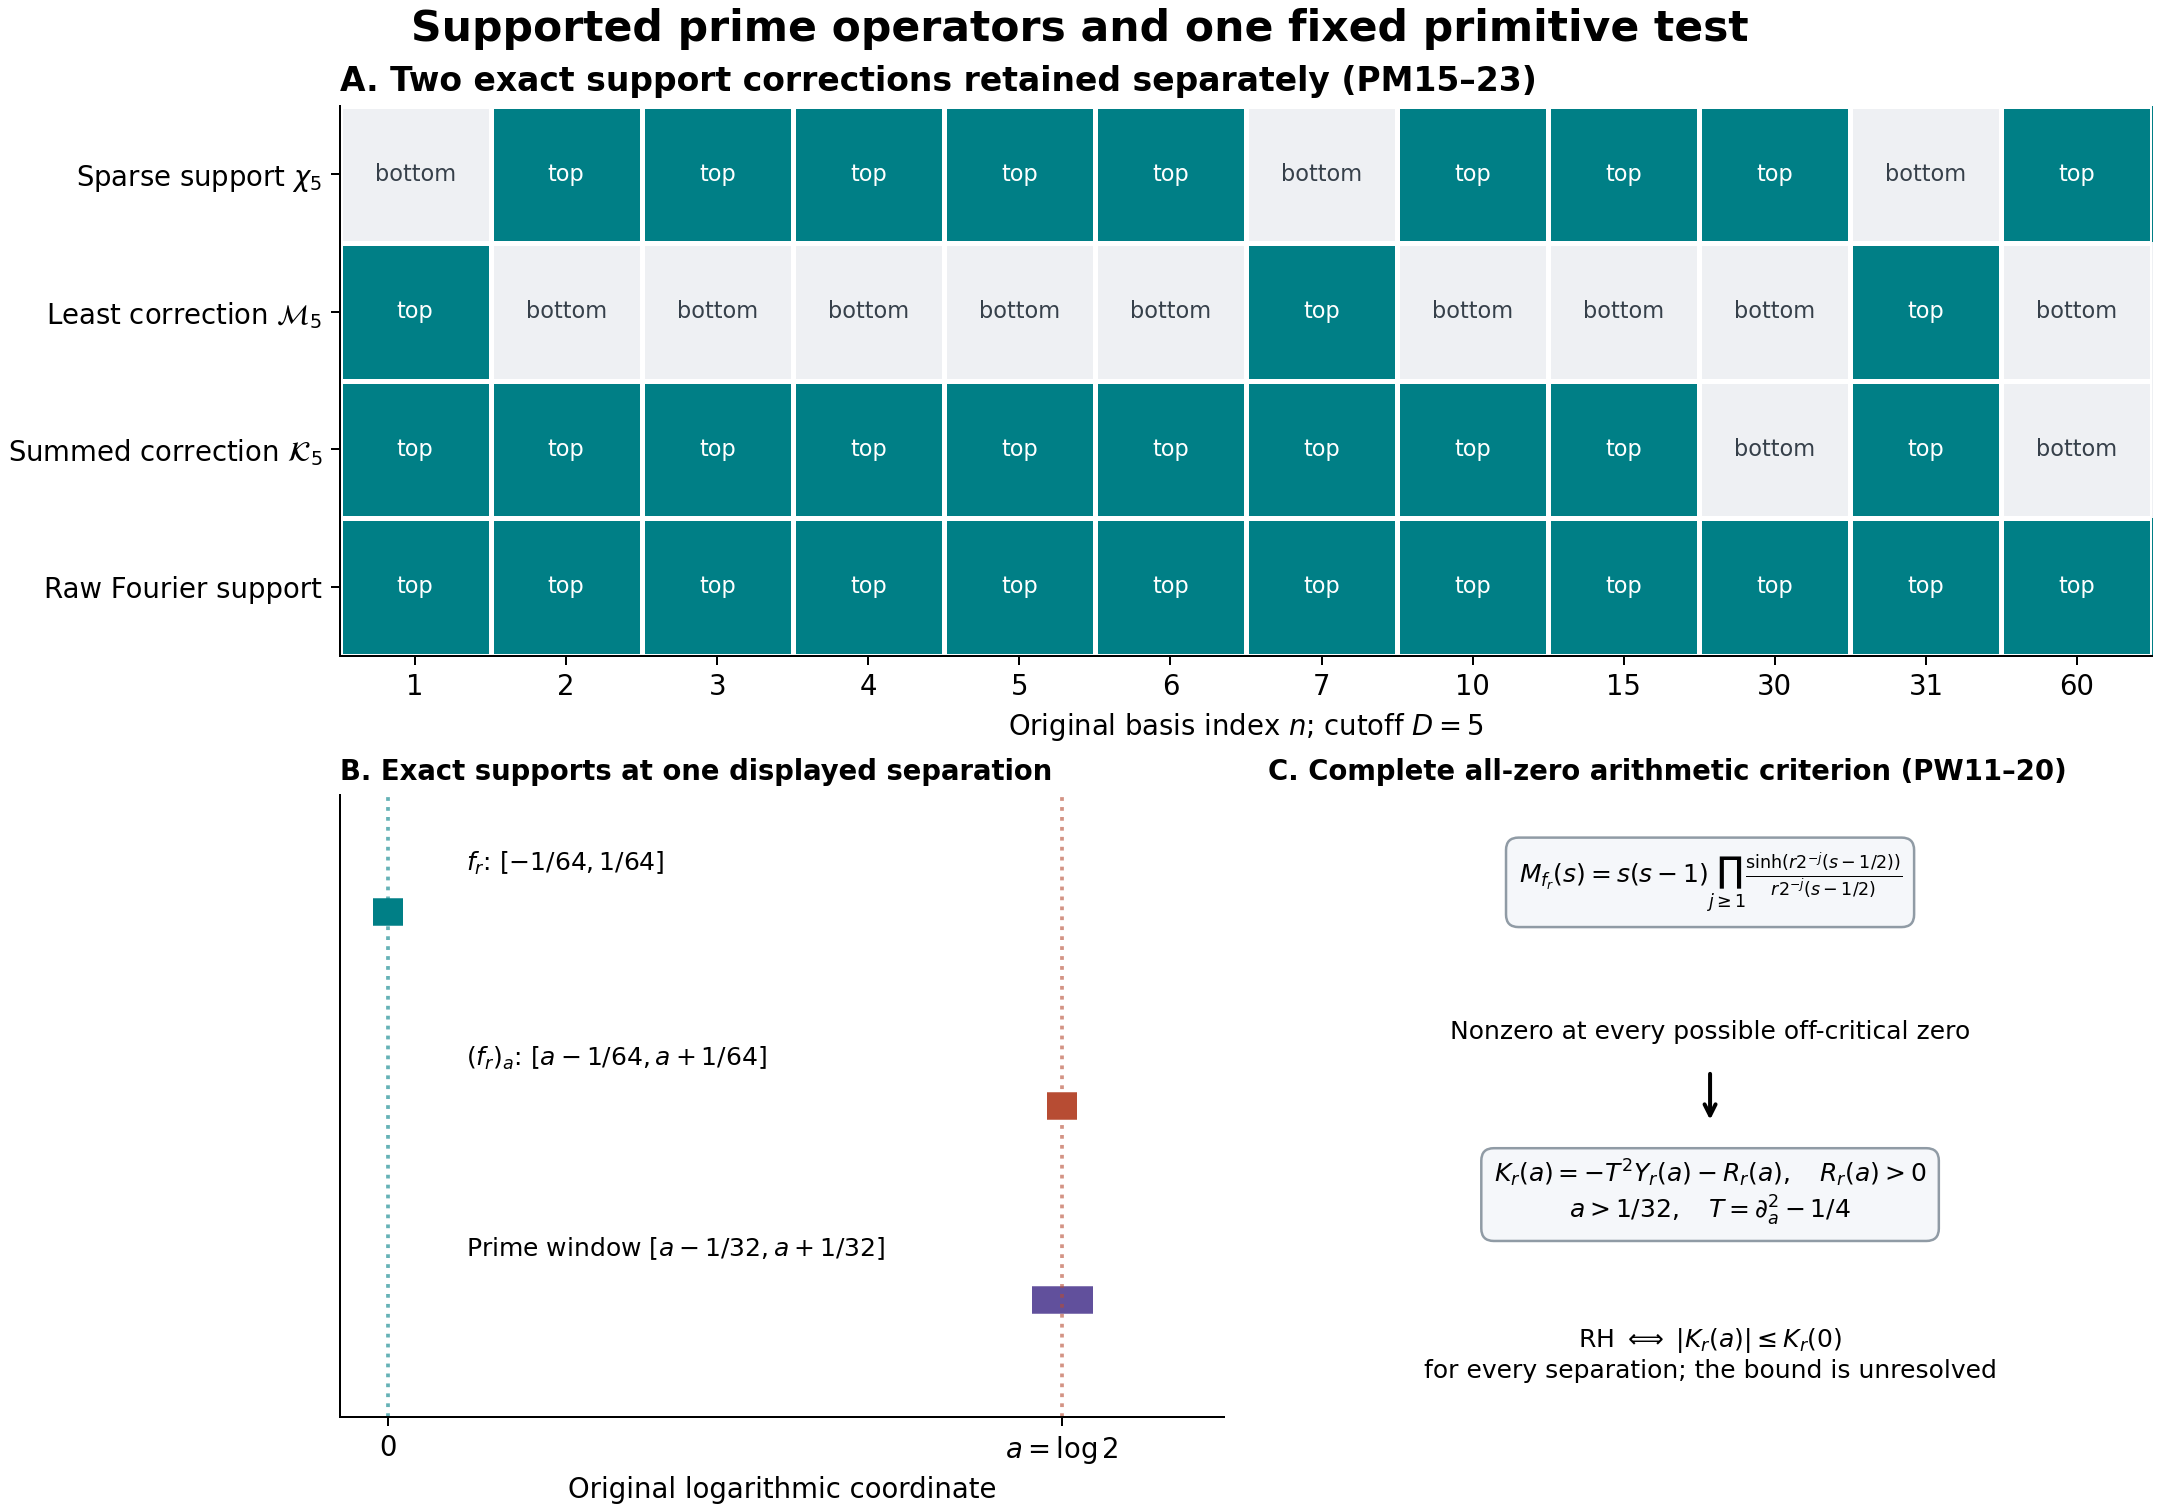
\includegraphics[keepaspectratio,alt={Exact support masks at cutoff five, the original test-support intervals and their prime window, and the complete criterion. The top panel shows all labels at the displayed indices, including the difference between the least correction and the directly summed Fourier correction. The middle support calculation uses the displayed separation a=log 2; the criterion concerns every separation. Proofs: PM15--23 and PW3--20. Both zero endpoint values retain supported-zero labels by PW21--22. The reproducible source draws the proved masks and interval coordinates; it does not sample a hypothetical zero.}]{primitive_prime_window.png}}
\caption{Exact support masks at cutoff five, the original test-support
intervals and their prime window, and the complete criterion. The top
panel shows all labels at the displayed indices, including the
difference between the least correction and the directly summed Fourier
correction. The middle support calculation uses the displayed separation
a=log 2; the criterion concerns every separation. Proofs: PM15--23 and
PW3--20. Both zero endpoint values retain supported-zero labels by
PW21--22. The reproducible source draws the proved masks and interval
coordinates; it does not sample a hypothetical zero.}
\end{figure}

\subsection{Proof sources and scope}\label{proof-sources-and-scope}

The analytic explicit formula and full support vector are the complete
SZW source cited above; the Gamma integral is HA13. Their original human
source includes Alain Connes,
\href{https://arxiv.org/abs/math/9811068}{\emph{Trace formula in
noncommutative geometry and the zeros of the Riemann zeta function}},
Appendix II, Theorem 6. The incoming BPZ proof supplies the
translation/Laplace method with all multiplicities; its full TeX is
included unchanged. The present fixed convolution, its complete analytic
construction, the short-support estimate, and PM's prime-operator
comparison have standalone proofs in this collection. These statements
specify their exact mathematical contribution without claiming priority
over the extensive classical literature on Weil criteria or smoothed
prime formulas.

\end{document}
